% the sample slide is created with 16:9 aspect ratio
\documentclass[aspectratio=169]{beamer}

% remove the options if you do not want to have them
\usetheme[
	% background=images/background.jpg, % you can add your own background image
	logo=images/unsw-portrait.png,
	sidelogo=images/unsw-landscape.png,
]{unsw}
\usepackage[compat=1.1.0]{tikz-feynman}
\usepackage[version=4]{mhchem}
\setbeamertemplate{caption}[numbered]
% uncomment to show notes. Works very nicely with dspdfviewer. You get something similar to PPT's presenter view.
%\usepackage{pgfpages}
%\setbeameroption{show notes on second screen}

% information for the title page
\author{Luke Wicent Sy}
\title{UNSW Beamer Theme}
\subtitle{An unofficial theme for University of New South Wales}
\institute{Graduate School of Biomedical Engineering}
\date{\today}

\begin{document}
	% use plain option to remove the page number from the title slide
	\begin{frame}[plain]
		\titlepage
	\end{frame}
	
	\begin{frame}{Introduction}
		Hello
	\end{frame}

	\begin{frame}{Overview}
		\tableofcontents
	\end{frame}

	\begin{frame}{Motivation}
		Convince you guys that the authors of both papers successfully managed to constrain the lower bound of the pair instability gap.
	\end{frame}

	\section{Stellar Theory}

	\begin{frame}{Stellar Theory}
		\begin{figure}
			\centering
			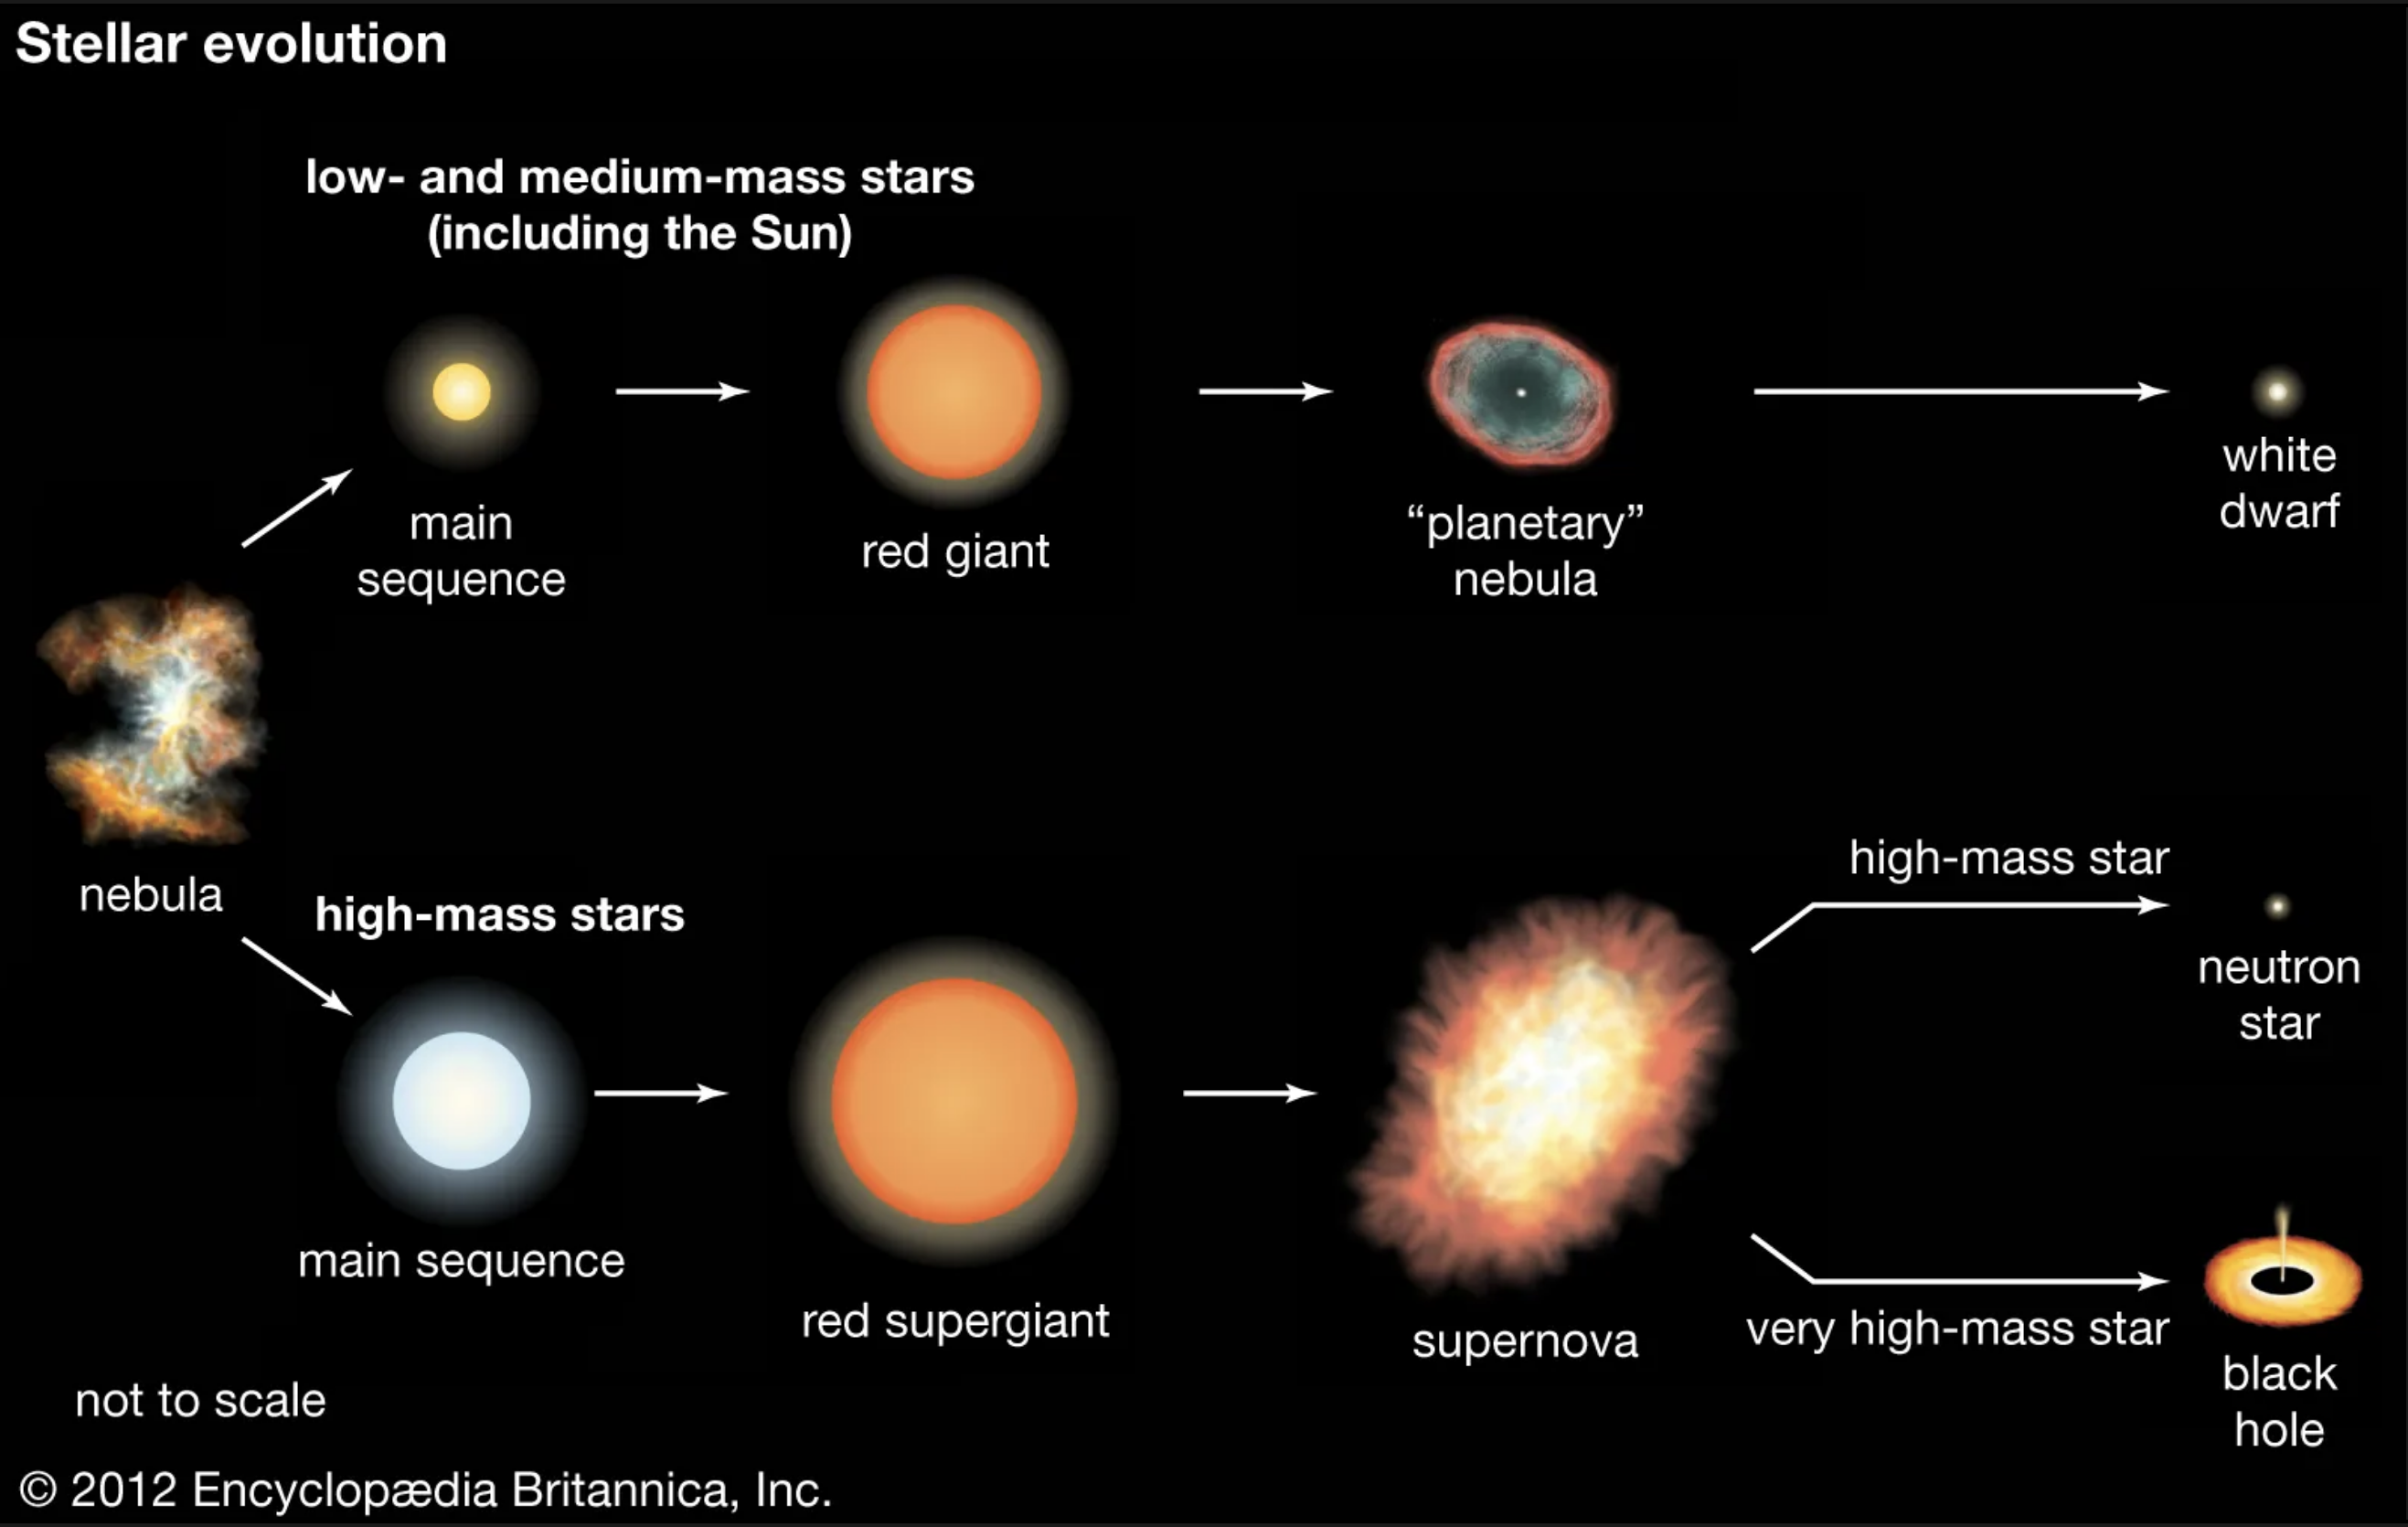
\includegraphics[width=0.6\textwidth]{images/starlifecycle.png}
			\caption{Britannica. High-mass star $M>3$ M$_\odot$. Very high-mass star $M>8$ M$_\odot$}
		\end{figure}
	\end{frame}

	\begin{frame}{Nuclear Processes}
		The main nuclear reaction in metal-poor or metal-free stars is the triple alpha process, which produces carbon, $3\alpha \rightarrow \ce{^{12}_6C}$. This carbon can be then be used for oxygen production,
		\begin{equation}
			\ce{^{12}_6C + ^{4}_2He -> ^{16}_8O + {\gamma}} 
		\end{equation}
		In astrophysical simulations of stellar evolution, the $S$-factor parameter or the $^{12}$C$(\alpha,\gamma)^{16}$O reaction rate, is important for modelling helium burning.
	\end{frame}

	\subsection{Pair Production instability}

	\begin{frame}{Pair Production}
		In supermassive stars, after sufficient helium and carbon are exhausted, the temperature in its core may get too high for stable oxygen production. Furthermore, the high energy gamma rays start producing electron-positron pairs, leading to instability of the star.

		\begin{figure}
			\centering
			\begin{tikzpicture}[scale=0.85, every node/.style={scale=0.85}]
				\begin{feynman}
					\vertex (a1) at (0,1.6) {\(\gamma\)};
					\vertex (v1) at (2,1.1);
					\vertex (a2) at (4,1.6) {\(e^-\)};
					\vertex (b1) at (0,-1.6) {\(\gamma\)};
					\vertex (v2) at (2,-1.1);
					\vertex (b2) at (4,-1.6) {\(e^+\)};

					\diagram* {
						(a1) -- [photon] (v1) -- [fermion] (a2),
						(v1) -- [fermion] (v2),
						(b1) -- [photon] (v2) -- [anti fermion] (b2),
					};
				\end{feynman}
			\end{tikzpicture}
			\caption{Pair production: $\gamma\gamma \to e^+e^-$}
		\end{figure}
	\end{frame}		

	\begin{frame}{Pair Instability Supernova}
		\begin{figure}
			\centering
			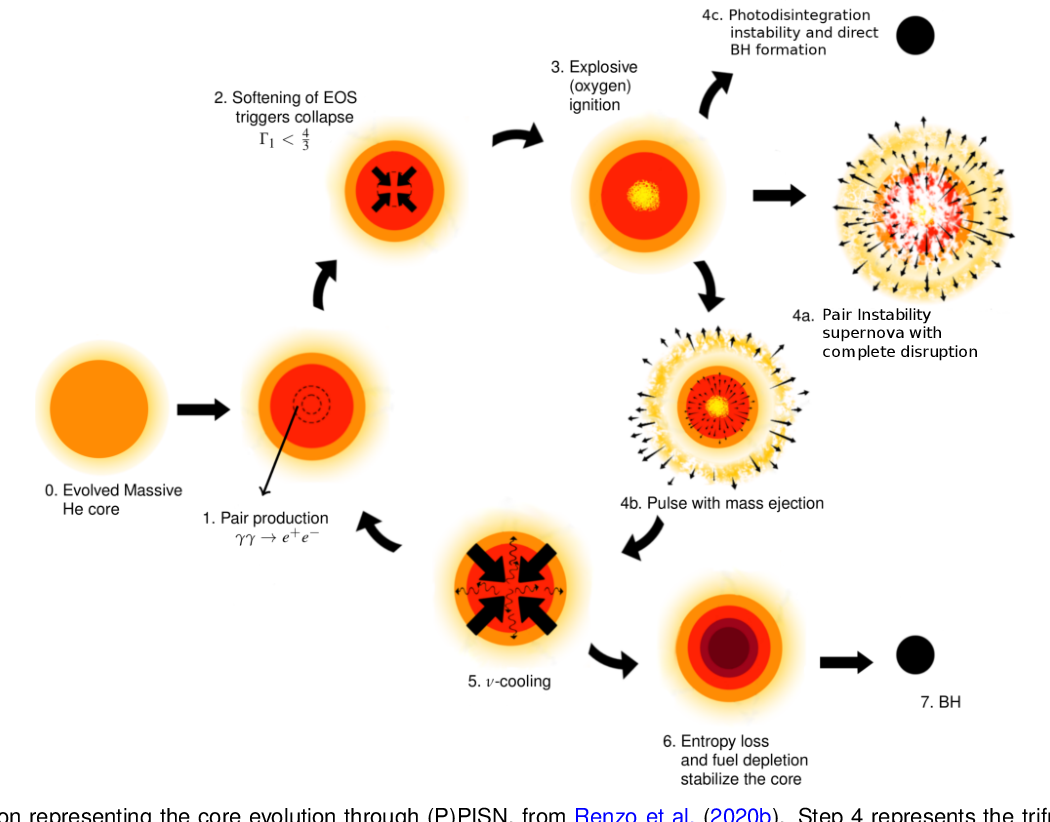
\includegraphics[width=0.5\textwidth]{images/SNEvolution.png}
			\caption{Binary}
		\end{figure}
	\end{frame}

	\subsection{Black hole mass gap}

	\begin{frame}{The black hole in black hole masses}
		\begin{columns}[t]
			\begin{column}[T]{0.6\textwidth}
				\begin{figure}
					\centering
					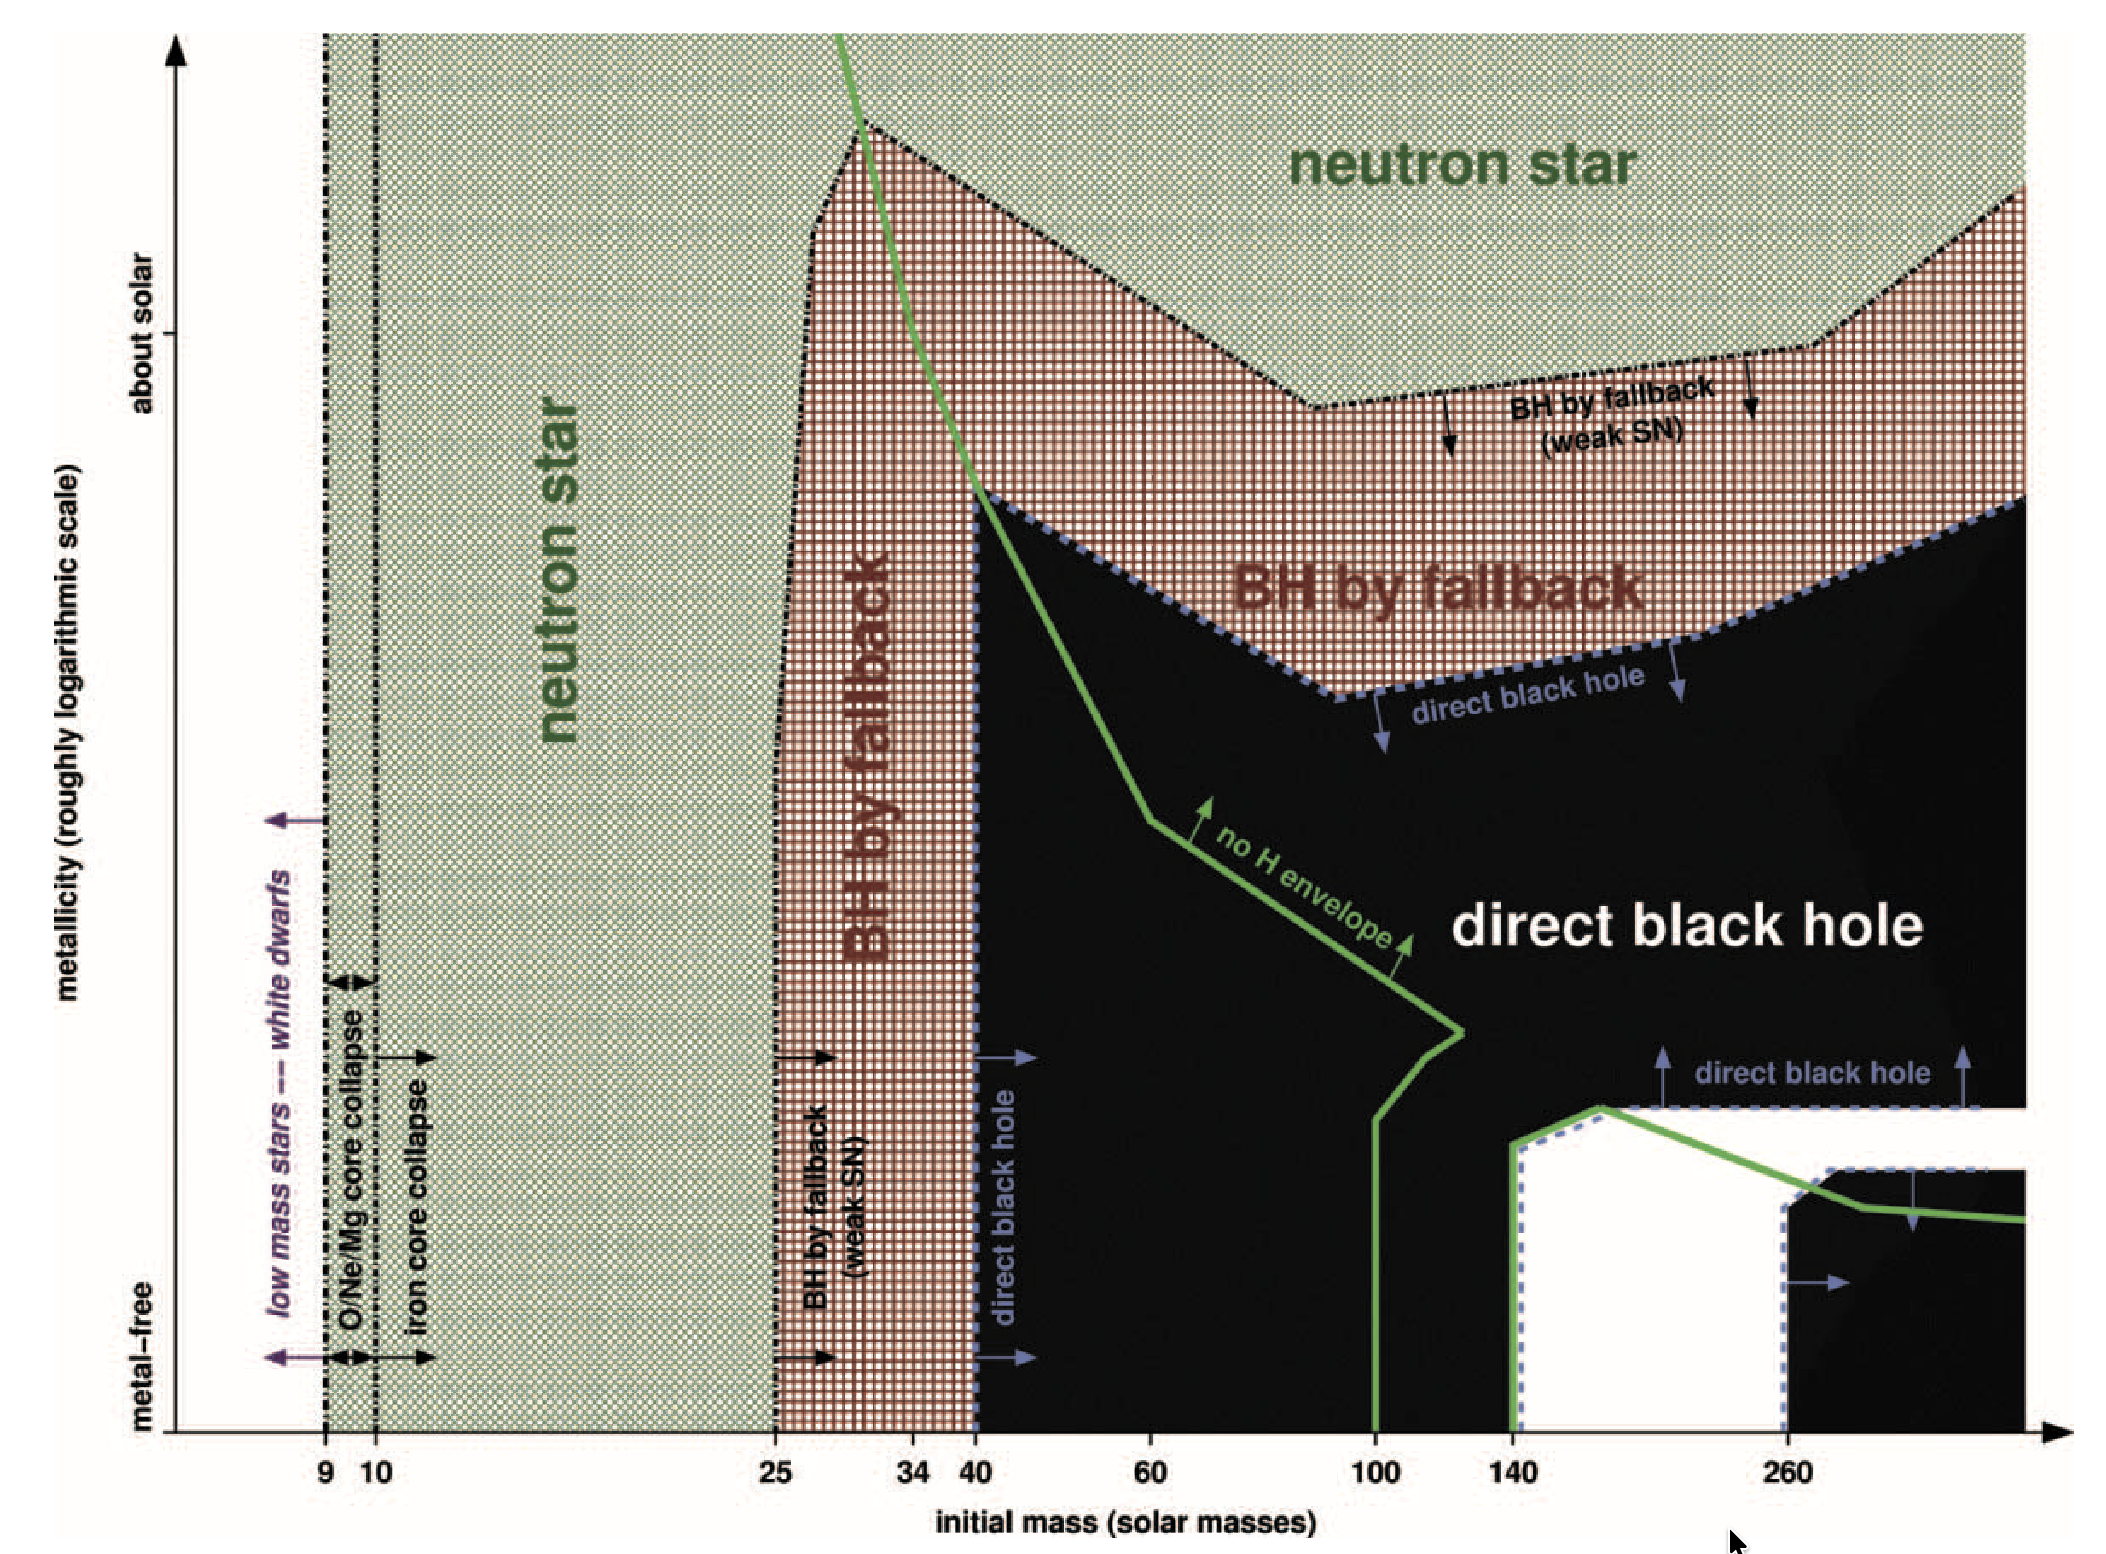
\includegraphics[width=0.8\textwidth]{images/BHGap.png}
					\caption{Phase diagram}
				\end{figure}
			\end{column}
			\begin{column}[T]{0.4\textwidth}
				\begin{itemize}
					\item In this column,
					\item we just add the
					\item bullet points.
				\end{itemize}
			\end{column}
		\end{columns}
	\end{frame}

	\subsection{Gravitational waves}

	\begin{frame}{Black hole spin}
		Solutions to the Einstein field equations predict that black holes can be described using angular momentum. 
		\begin{itemize}
			\item Known as a Kerr black hole
			\item These rotating black holes can form from collisions or merging with spinning objects such as stars or gas.
			\item The Kerr metric is parameterised with angular momentum, $\chi$.
			\item In the limit of $\chi\rightarrow 0$, the Kerr metric reduces to the Schwarzschild metric.
		\end{itemize} Black hole merger remnants are expected to have nearly universal spin magnitude 
		\begin{equation}
			\chi = a_{\text{rem}} \approx 0.7
		\end{equation}
	\end{frame}

	\begin{frame}{Binary systems and gravitational waves}
		\begin{figure}
			\centering
			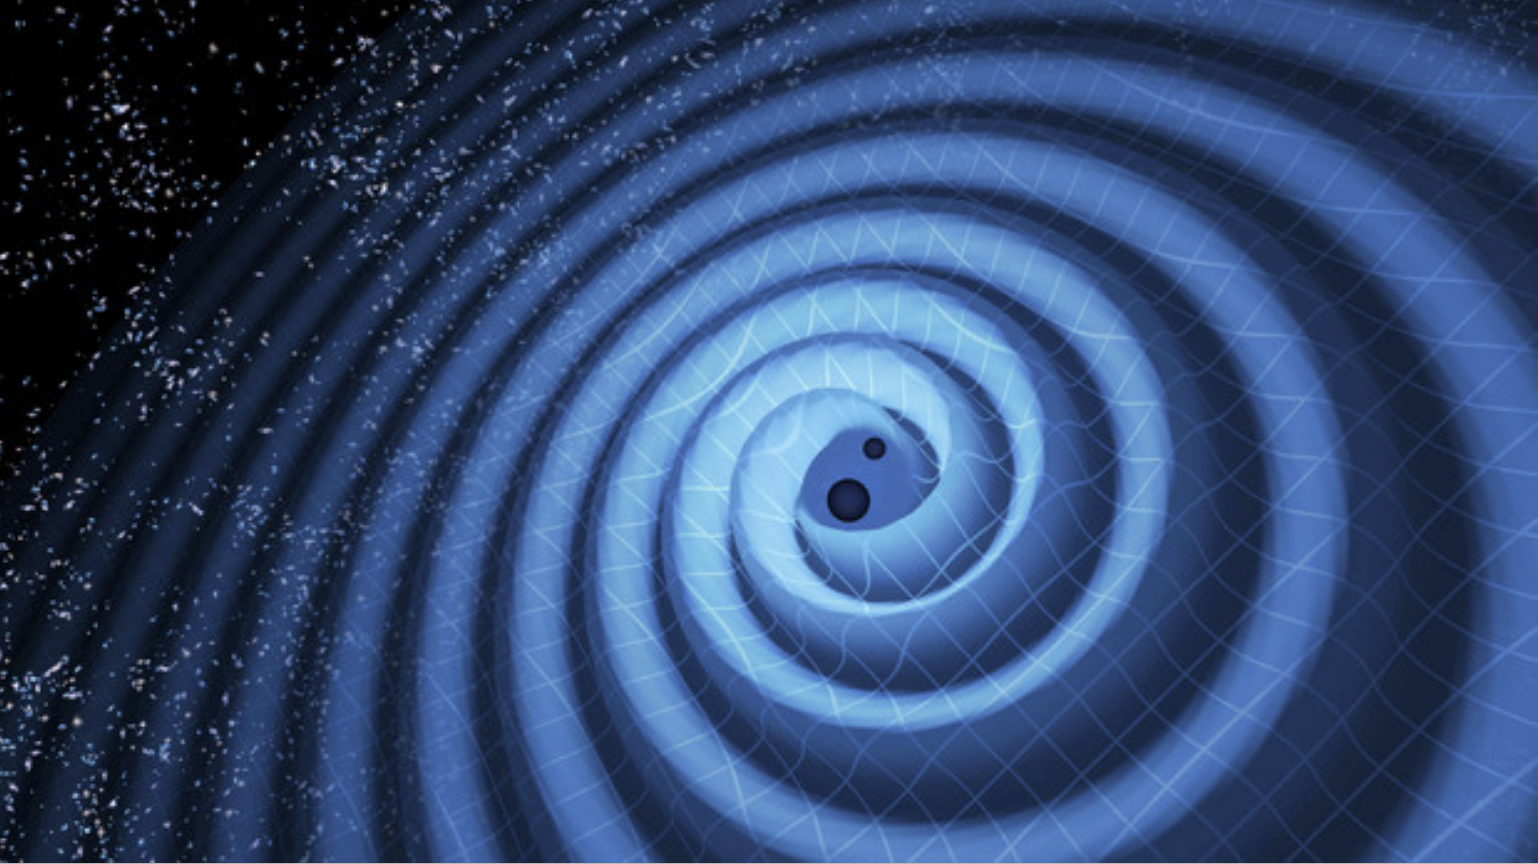
\includegraphics[width=0.7\textwidth]{images/binary.png}
			\caption{Binary}
		\end{figure}
	\end{frame}

	\section{LIGO-Virgo-KAGRA}

	\begin{frame}{Gravitational waves interferometry}
		\begin{columns}[t]
				\begin{column}[T]{0.6\textwidth}
				\begin{itemize}
					\item A simple interferometer set up measures the \textit{strain} caused by a gravitational wave. The strain is defined as the contraction or expansion over the distance travelled
					\begin{equation}
						h = \frac{\Delta x}{L}
					\end{equation}
					\item The strain of 2 orbiting 10 M$_\odot$ black holes is on the order of $\mathcal{O}\left(10^{-22}\right)$
					\item This wave could distort the Earth by $10^{-15}$ m or $0.01\%$ the size of the atom.
				\end{itemize}
			\end{column}
			\begin{column}[T]{0.4\textwidth}
				\begin{figure}
					\centering
					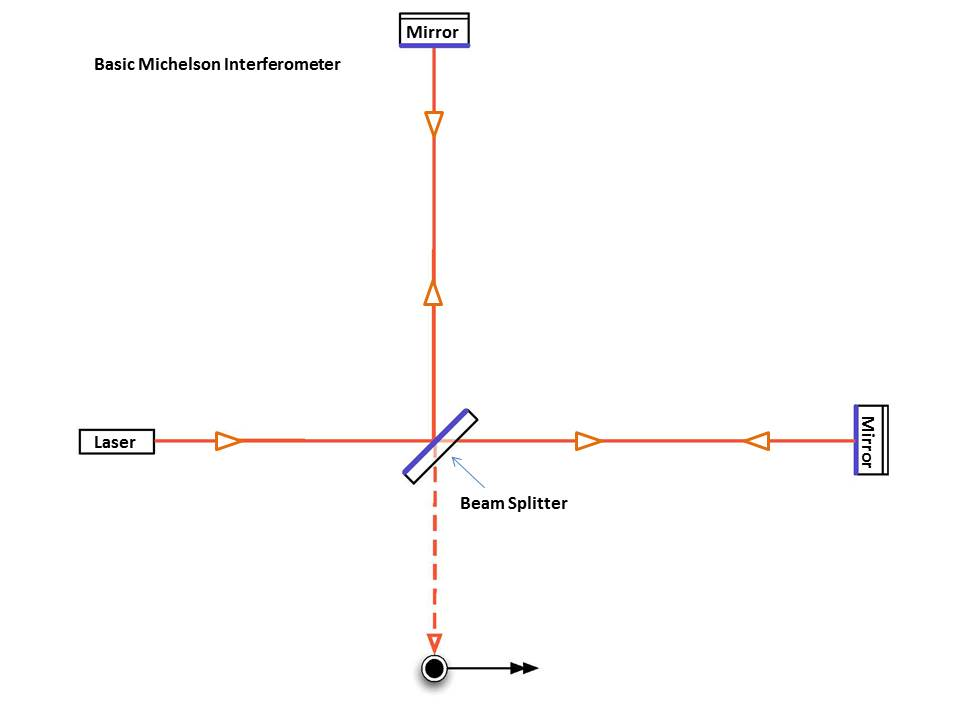
\includegraphics[width=0.8\textwidth]{images/interferometer.png}
					\caption{Phase diagram}
				\end{figure}
			\end{column}
		\end{columns}
	\end{frame}

	\begin{frame}{LIGO-Virgo-KAGRA}
		The Gravitational Wave Transients Catalog (GWTC) is consists of data obtained by three interferometers: LIGO, Virgo and KAGRA. 
		\begin{itemize}
			\item LIGO has two observatories based in the US. Each interferometer has mirrors spaced 4 km apart in order to measure changes in length of less than one ten-thousandth the charge diameter of a proton.
			\item Virgo (Italy) and KAGRA (Japan) have interferometers with mirrors spaced 3 km apart.
		\end{itemize}
		The newest catalog, GWTC-4, provides the mass and effective spin from 153 events.
	\end{frame}

	\begin{frame}{Instruments}
		\begin{columns}[t]
			\begin{column}[T]{0.5\textwidth}
				\begin{figure}
					\centering
					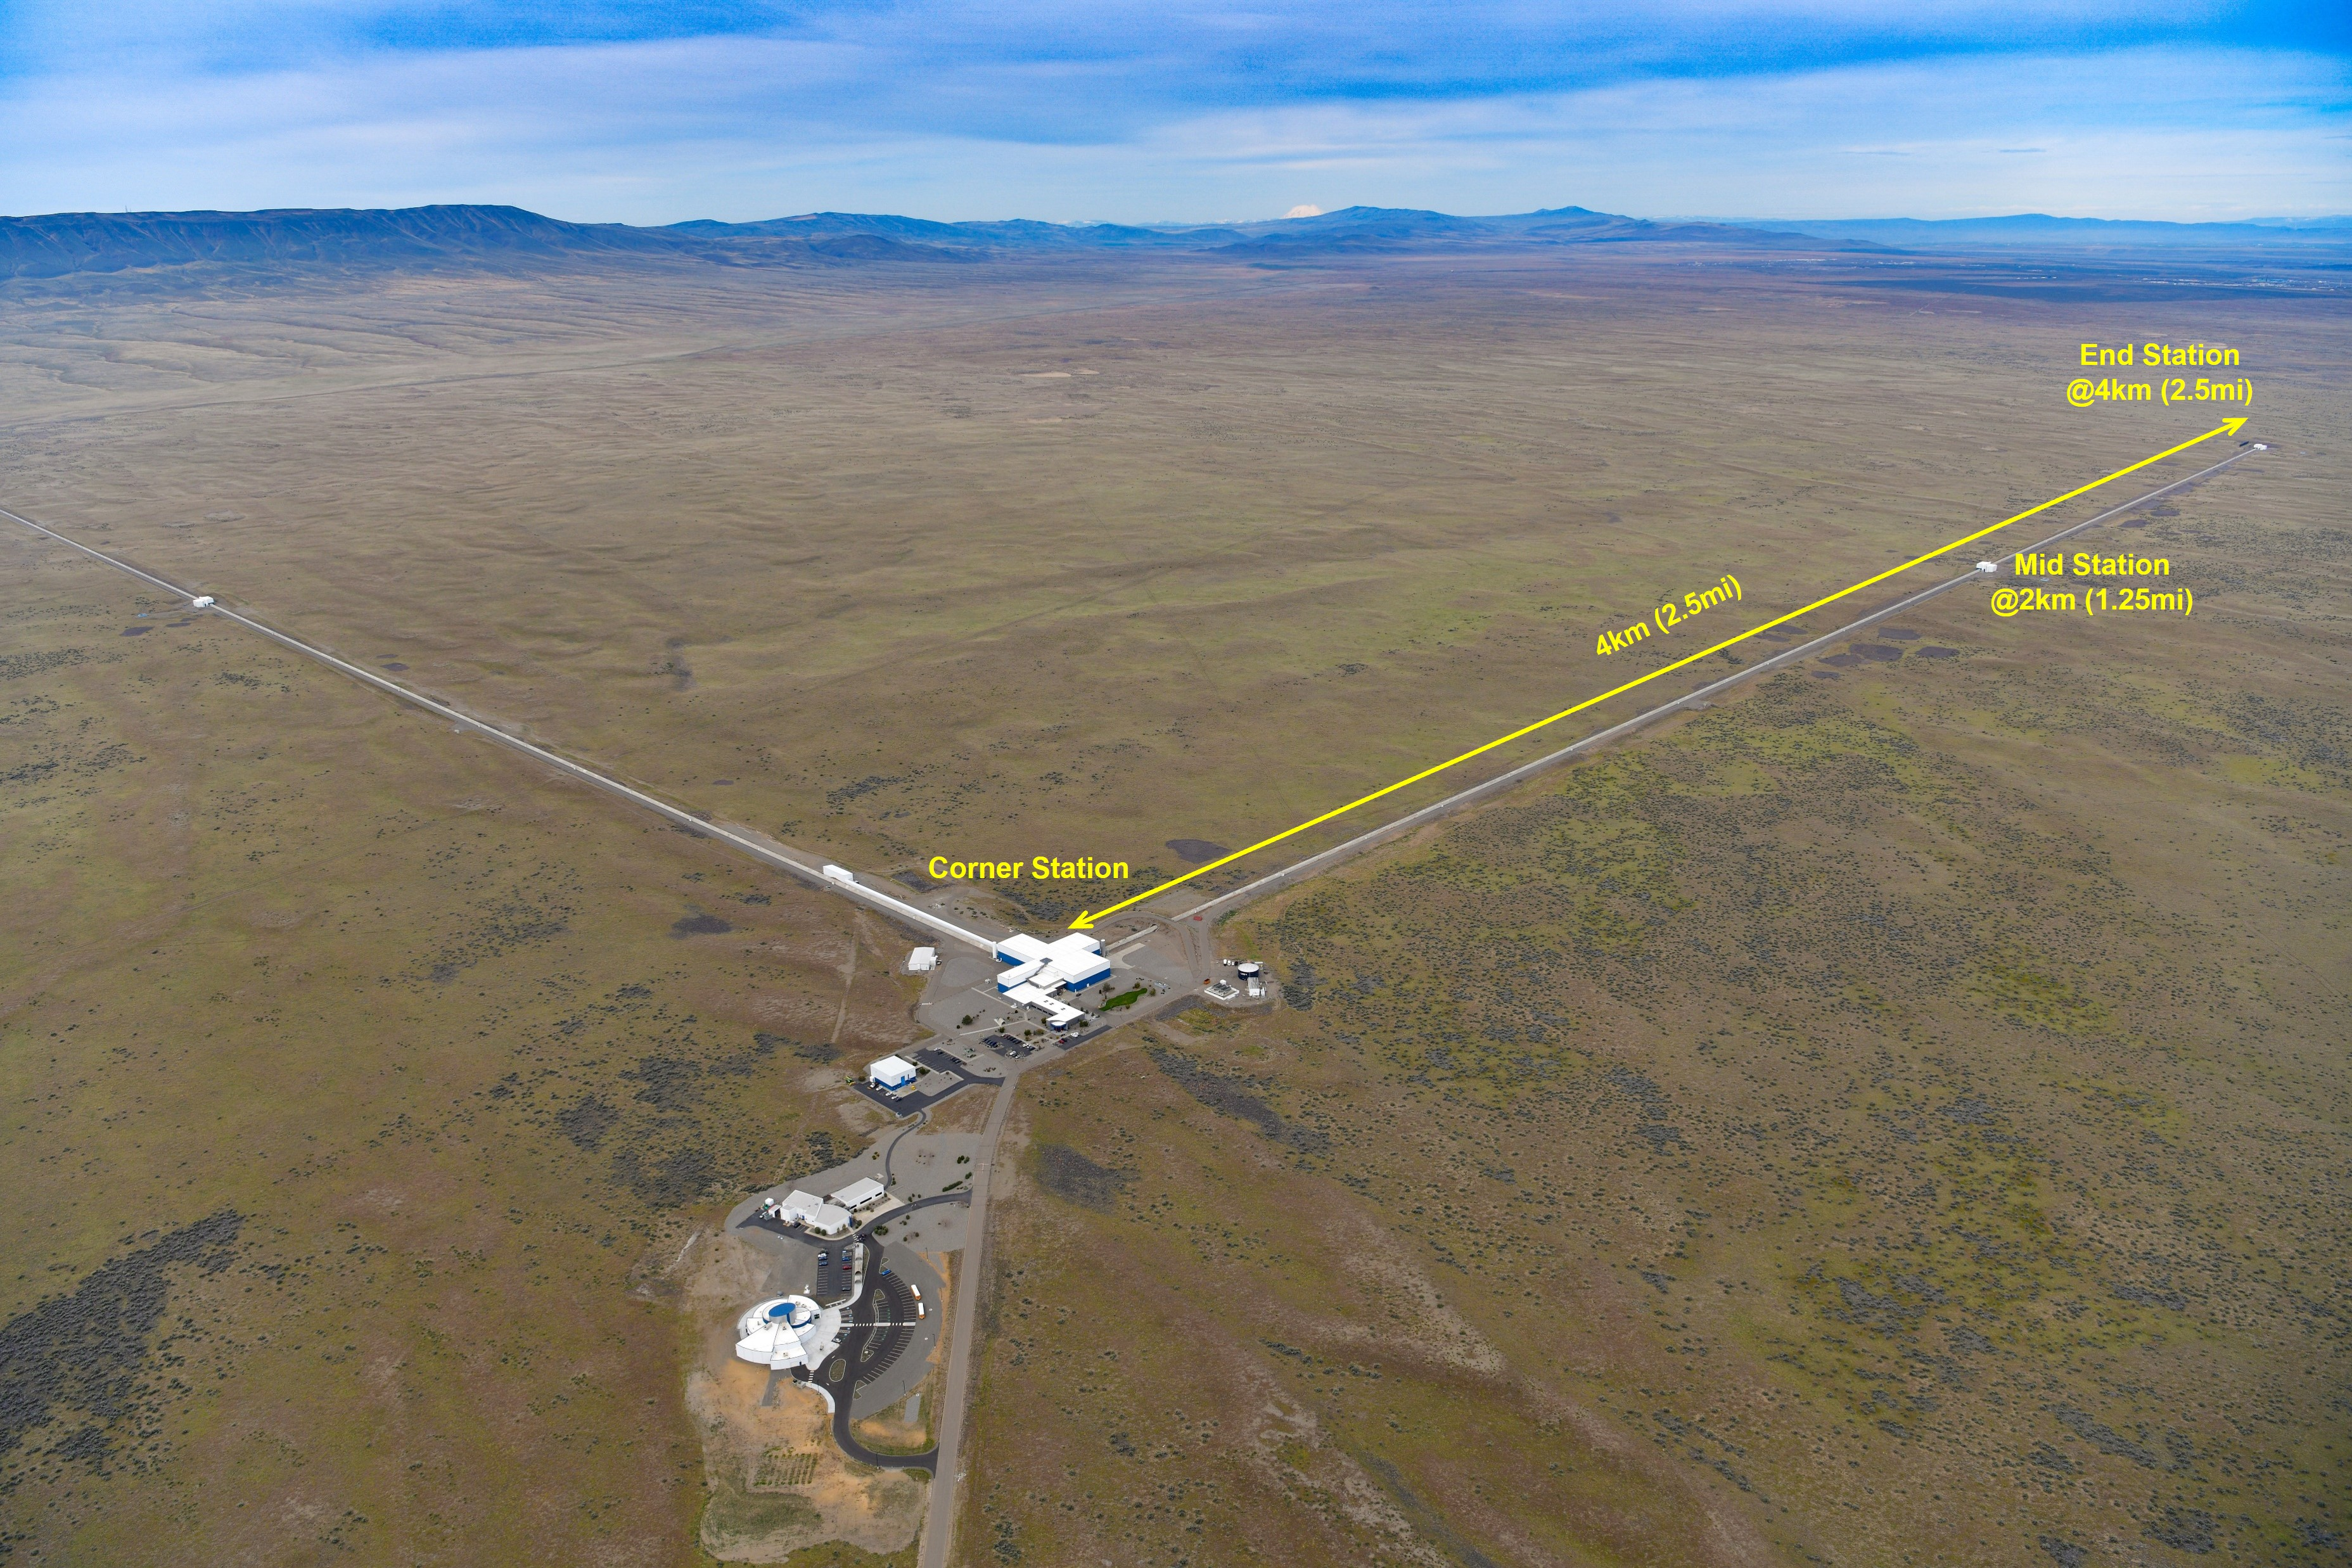
\includegraphics[width=\textwidth]{images/ligo.jpg}
					\caption{Phase diagram}
				\end{figure}
			\end{column}
			\begin{column}[T]{0.5\textwidth}
				\begin{figure}
					\centering
					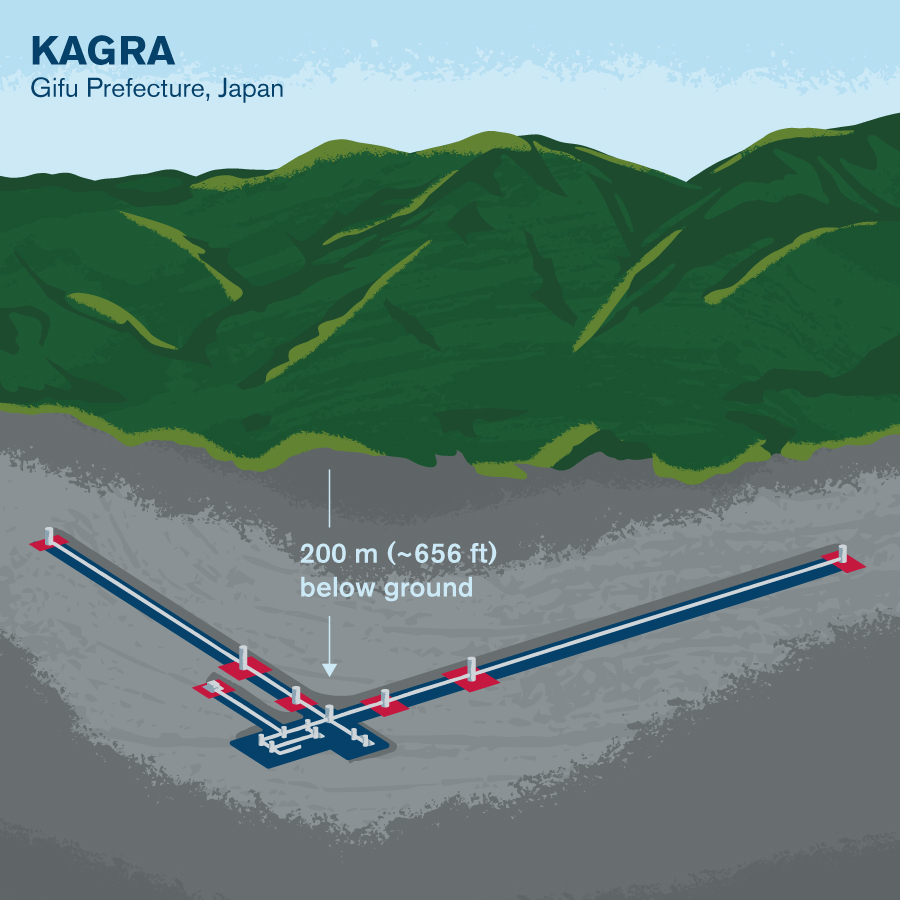
\includegraphics[width=0.8\textwidth]{images/kagra.jpg}
					\caption{Phase diagram}
				\end{figure}
			\end{column}
		\end{columns}
	\end{frame}

	\section{Achievements}
	\begin{frame}{Novel findings}
		Both papers agree on the lower bound of the mass gap and the reaction rate. They provide contraints on these parameters enabling better models for stellar evolution. The innovation of these papers are:
		\begin{itemize}
			\item Tong shows that the gap only appears in the secondary mass of a binary system. Previous studies only showed that hierachical mergers fill the gap and were unable to separate the two components of the system like Tong does.
			\item Antonini verifies a prediction made by general relativity by fixing a universal parameters and developing a model to predict the existence of the gap based on just one fixed assumption.
		\end{itemize}
	\end{frame}

	\begin{frame}{Impact on physics}
		If the $^{12}$C$(\alpha,\gamma)^{16}$O reaction rate was precisely measured then:
		\begin{itemize}
			\item The ratio of $^{12}$C/$^{16}$O in the universe can be determined
			\item This reaction is responsible for the production of oxygen in the universe
			\item Reveals the nucleosynthesis process in the first stars 
		\end{itemize}
		The pair instability gap can be used as a \textit{standard siren}
		\begin{itemize}
			\item The gravitational waveform can carry information about the distance
			\item This enables better measurements for the rate of universe expansion and the Hubble parameter.
		\end{itemize}
	\end{frame}

	\begin{frame}{Appendix}
		Appendix
	\end{frame}

	\begin{frame}{Different types of stars}
		There are three distinct classifications of stellar populations:
		\begin{itemize}
			\item The mass range for Population I \& II stars is $0.08-150$ M$_\odot$ 
			\item Population I stars are younger, metal-rich.
			\item Population II stars are older, metal-poor but rich in alpha-elements.
			\item Population III stars are hypothesised to be the oldest and largest stars, metal-free. The typical mass range for these stars could be $\sim 100 - 300$ M$_\odot$.
		\end{itemize}
	\end{frame}

	\begin{frame}{Nuclear processes and supernova}
		Type Ia supernova
		\begin{itemize}
			\item Occurs in binary star systems where one massive star becomes an accreting white dwarf. Once the dwarf reaches the Chandrasekhar limit (1.44 M$_\odot$), igniting the carbon fusion causing a thermonuclear explosion.
			\item The supernovae has uniform properties (light curve is consistent) and thus are useful standard candles.
		\end{itemize}
		Type II supernova
		\begin{itemize}
			\item Occurs in very massive stars, the nuclear fusion becomes unable to sustain the core against its own gravity.
			\item Core collapse can be caused by different mechanisms: exceeding the Chandrasekhar limit, electron capture, pair-instability or photodisintegration.
		\end{itemize}
		The most luminous supernovae (superluminous supernova) are speculated to be pair-instability supernova (PISN). They are atleast 10 times as bright as standard supernova.
	\end{frame}

\end{document}
